% ============================= Evaluation ============================
\section{Evaluation}
\label{sec:evaluation}

We have applied our approach to four SPLs: the eShop Product Line, as partially
shown  in Section~\ref{sec:svmc}; the Pedagogical Product Line
(PPL)~\cite{PPL:2008}, which was proposed for learning about and experimenting
with software product lines, and focuses on the arcade game domain; the Smart
Home Product Line, based on different
specifications~\cite{Pohl:2005aa,Alferez:2008aa}, and the Multimedia Message
Product Line (MMS), a case study conducted with one of our industrial partners.

The last one---which consists of products for creating, sending, and receiving
multimedia messages (MMS) in mobile phones---was used to evaluate an early
version of our approach~\cite{Bonifacio:2008aa}, using Design Structure Matrices
(DSMs) and a suite of metrics for quantifying
specification modularity and complexity. Here, we use it again, but with an
improved metric suite and a new method for assigning features to scenarios steps. In this paper we focused our comparisons with
the PLUSS approach, mainly because in a previous work we have identified that PLUC specifications are not maintainable at all~\cite{Bonifacio:2008aa}. Even the introduction of a new member in the SPL require changes in many PLUC scenarios.

It is important to note that each case study was conducted with different
settings. For instance, groups of students were assigned to specify the behavior
of the Smart Home product line in both PLUSS and MSVCM techniques. Differently, we
compared our approach to an available PLUSS specification of the PPL. The input
data and the tasks performed in each case study were also different. For example,
some of the case studies (Smart Home and MMS) started from the specification of
different products of a family. On the other hand, both \emph{eShop} and PPL case
studies started from existing product line specifications. Next, we first present this new metric suite,
and then describe the assessment of the Smart Home, MMS, and PPL case studies. 


\subsection{Metric suite}\label{sub:metric-suite}

In order to evaluate our approach, we customized the metric suite proposed by Eaddy et al.~\cite{Eaddy:2007aa},
considering the degree of scattering of features and the degree of focus of scenarios. We also customized their \emph{prune dependency analysis}, as a guide to
assign features to scenario steps. Actually, we consider that a step $s$ depends on a feature $f$ iff the configuration of $f$ effects the selection or the configuration of the step $s$. Therefore, we name our assignment approach
\emph{configuration dependency analysis}.  The \emph{degree of scattering} of a
feature $f$ is calculated by normalizing its concentration with respect to each
scenario $s \in S$ (the set of all scenarios).



%
%We can now explain the semantics of both metrics (degree of scattering and
%degree of focus) used in this work. First, the \emph{degree of scattering} of a
%feature $f$ is calculated by normalizing its concentration with respect to each
%scenario $s \in S$ (the set of all scenarios).

\begin{center}
$DOS(f) = 1 - \frac{\mid S \mid \sum_{s}^{S}(CONC(f,s)-\frac{1}{\mid S
\mid})^2}{\mid S \mid -1}$, where:

$CONC(f,s) = \frac{number\ of\ steps\ in\ s\ assigned\ to\ f}{total\ number\
of\ steps\ assigned\ to\ f}$
\end{center}

Likewise, the \emph{degree of focus} of a scenario $s$ is calculated by
normalizing its dedication with respect to each feature $f \in F$ (the set of
all features).

\begin{center}
$DOF(s) = \frac{\mid F \mid \sum_{f}^{F}(DEDI(s,f)-\frac{1}{\mid F
\mid})^2}{\mid F \mid -1}$, where:

$DEDI(s,f) = \frac{number\ of\ steps\ in\ s\ assigned\ to\ f}{total\ number\
of\ steps\ in\ s}$
\end{center}

These metrics inherit the same properties of the original
ones~\cite{Eaddy:2007aa}: (a) the
\emph{degree of scattering} (DoS) is normalized between 0 (completely localized)
and 1 (completely unlocalized); and (b) the \emph{degree of focus} (DoF) is also
normalized between 0 (completely unfocused) and 1 (completely focused).


For instance, consider the scenarios shown in
Figure~\ref{fig:smartHomeScenarios}, which represents the assignment of a few Smart Home features to 
both PLUSS and MSVCM specifications. The left hand side of
Figure~\ref{fig:smartHomeScenarios}(a) depicts that the PLUSS specification of
Register Inhabitant scenario has seven steps. Two of these steps were assigned only to the \emph{Register Inhabitant} (RI) feature; other two steps
were assigned to the interactions between \emph{Register Inhabitant} and
\emph{Password} features; and other three steps were assigned to the
interactions between \emph{Register Inhabitant} and \emph{Fingerprint}
features. Notice that the \emph{Password} and \emph{Fingerprint} features, which
are mutually exclusive, also change the behavior of the \emph{Request Access to
Home} feature (Figure~\ref{fig:smartHomeScenarios}(b)).


\begin{figure}[th]
 \begin{center}
  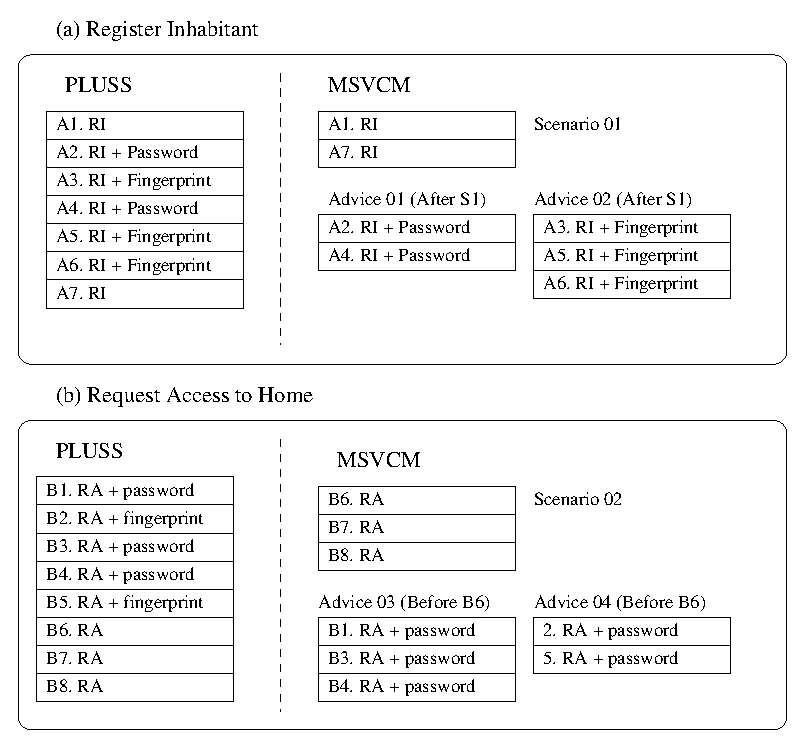
\includegraphics[scale=0.65]{img/comparisonScenarios.eps}
  \caption{Sample of Smart Home assignments.}
  \label{fig:smartHomeScenarios}
  \end{center}
\end{figure}

Similarly, Figure~\ref{fig:MMSScenarios} shows some feature assignments for the
MMS product line. In this case, we want to emphasize that the behavior related to
the \emph{Store an Embedded Number} and \emph{Send a Message to Embedded Email} 
features change the behavior of the \emph{Receive a MMS} and \emph{Select a
MMS for Displaying} features in a similar way. For this reason, we
classify the behavior of the \emph{Store an Embedded Number} and \emph{Send
a Message to Embedded Email} features as \emph{homogeneous}. On the other hand,
we say that the \emph{Password} optional feature of the Smart Home case study has a
\emph{heterogeneous crosscutting behavior}~\cite{Apel:2006aa}, since it requires one advice for each join point (Figure~\ref{fig:smartHomeScenarios}(a) and (b)). The same occurred with the \emph{Fingerprint} feature.

\begin{figure}[hbt]
 \begin{center}
  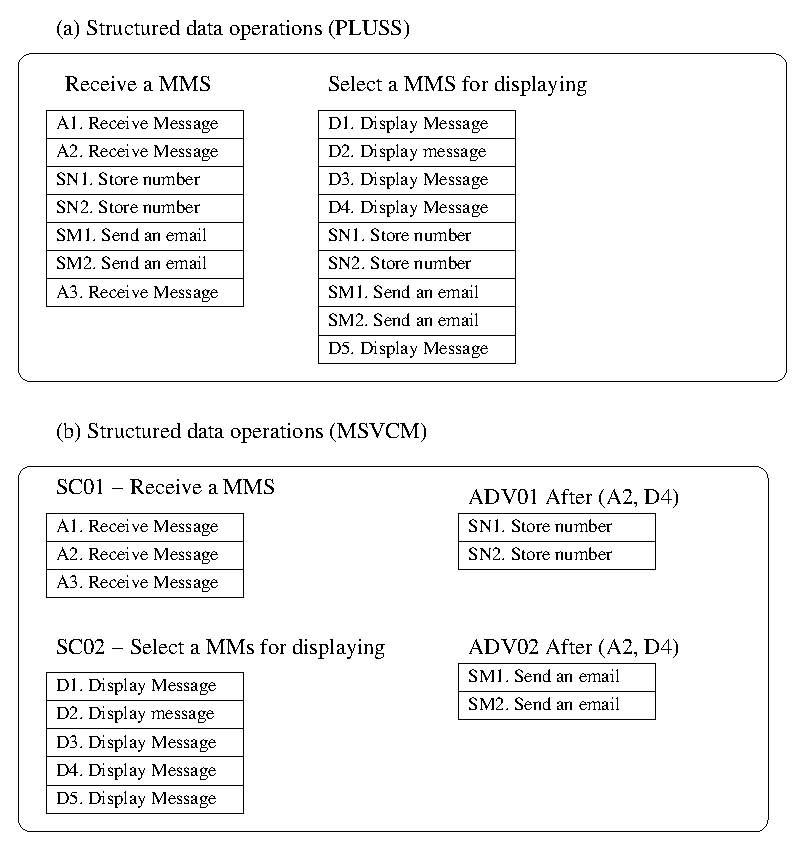
\includegraphics[scale=0.65]{img/comparisonScenarios2.eps}
  \caption{Sample of MMS assignments.}
  \label{fig:MMSScenarios}
  \end{center}
\end{figure}

We have observed that the \emph{crosscutting nature} of a feature, which here we
consider as being homogeneous or heterogeneous~\cite{Apel:2006aa}, has a great influence in our
results. For instance, Table~\ref{tab:feature-dos} shows the DoS of
the assets depicted in Figures~\ref{fig:smartHomeScenarios}
and~\ref{fig:MMSScenarios}. Notice that, in MSVCM, modularizing the behavior
of \emph{Password} and \emph{Fingerprint} as advices had
increased the DoS of both \emph{Register Inhabitant} and \emph{Request Access to
Home} features. A similar problem does not occur with homogeneous
crosscutting features--- modularizing the
\emph{Store an Embedded Number} and \emph{Send Message to Embedded Email} as advices does not 
change the DoS of the \emph{Receive a MMS} and \emph{Select a MMS for Displaying} features.    

\begin{table}[thb]
\centering
\caption{DoS of the presented features}
\label{tab:feature-dos}
\begin{small}
\begin{tabular}{p{0.25in}lll} \hline
SPL							&	Feature						& PLUSS	& MSVCM	\\ \hline 
 							&	Register Inhabitant				& 0.00  & 0.57  \\
Smart						&	Request Access to Home			& 0.00  & 0.57  \\ 
Home						&	Password						& 0.96  & 0.78  \\ 
							&	Fingerprint					& 0.96  & 0.78  \\ \hline
\multirow{4}{*}{MMS}	 		&	Receive a MMS				& 0.00  & 0.00  \\ 
							&	Select a MSS for Displaying		& 0.00  & 0.00  \\ 
							& 	Store an Embedded Number		& 1.00  & 0.00  \\
							& 	Send a Message to Email			& 1.00  & 0.00  \\ \hline		
\end{tabular}
\end{small}
\end{table}

Besides that, independently of the crosscutting nature of a feature, the
MSVCM approach eliminates the tangling of the base scenarios, quantified by
the DoF metric. As shown in Table~\ref{tab:scenario-dof}, the base scenarios in
MSVCM have a higher degree of focus. 

In what follows, we present summaries of the data collected from the
aforementioned case studies. Since each case study presents a different distribution of
\emph{crosscutting features}, the significance level related to the benefits
of our approach vary. All specifications and collected data are available~\cite{SPG:site}.


\begin{table}[htb]
\centering
\caption{DoF of the presented scenarios}
\label{tab:scenario-dof}
\begin{small}
\begin{tabular}{llll} \hline
SPL							&	Scenario		& PLUSS	& MSVCM	\\ \hline
\multirow{2}{*}{Smart Home} &	Scenario 01		& 0.24  & 1.00  \\
							&	Scenario 02		& 0.27  & 1.00  \\ \hline
\multirow{2}{*}{MMS} 		&	Scenario 01		& 0.12  & 1.00  \\ 
							&	Scenario 02		& 0.20  & 1.00  \\ \hline
\end{tabular}
\end{small}
\end{table}

\subsection{Smart Home assessment}

This study aimed at comparing feature modularity of PLUSS and MSVCM
specifications. Initially, three different products of the security module of a
Smart Home family~\cite{Pohl:2005aa} were specified. Almost six use cases and
fifteen scenarios are present in each product, with a significant number of
duplicated steps among them. These specifications, available on-line, were used
as input data. Then, six students, organized in groups, were assigned to identify
the commonalities and variabilities among the products, and to restructure the
input specifications. Two SPL specifications were produced, one using the PLUSS
notation and the other one using the MSVCM approach

%This study was divided in four major phases: (1) the specification of the input
%data --- three different configurations of the security module of a smart home
%were specified without PL support; (2) the presentation of preparatory classes to the subjects
%(graduate students with similar skills in the area); (3) the activity of
%restructuring the input specifications using both PLUSS and the Crosscutting
%technique; and (4) the assessment of the resulting specifications.
%In the first phase we have specified three different configurations of the
%security module of a Smart Home. These specifications included feature models and
%use case scenarios written without product line support. Additionally, they were
%build upon the documentation available from~\cite{Pohl:2005aa,AMPLE}.

%In the second phase, introductory classes and bibliographic references were
%offered to post-graduate students. At that period, none of these students had had
%previous knowledge in the field of scenario variability management. A total of
%six students were involved in this case study. Then, the students were organized
%in groups and assigned to restructure the input specifications using PLUSS and
%Crosscutting techniques.


Table~\ref{tab:sh-dos} summarizes the resulting \emph{degree of scattering} of
the Smart Home features, computed from the PLUSS and MSVCM specifications.
Although the MSVCM approach achieved a central tendency (median) closer to
zero, for some features (3 features in a total of 17) the DoS for the MSVCM approach
presented a greater value than the corresponding ones in PLUSS.


\begin{table}[htb]
\centering
\caption{Smart Home degree of scattering}
\label{tab:sh-dos}
\begin{small}
\begin{tabular}{llllll} \hline
					& Min 	& Median 	& Mean 	& Max 	& St. Deviation \\ \hline 
	PLUSS			& 0.00  & 0.26   	& 0.28  & 0.70 	& 0.08 			\\
	MSVCM	& 0.00  & 0.00  	& 0.26 	& 0.82 & 0.10  		\\ \hline	
\end{tabular}
\end{small}
\end{table}

As discussed in the previous section, modularizing the variant behavior of
\emph{Register Inhabitant} and \emph{Request Access to Home} in advices produced the side effect of increasing the DoS, at the same time that it reduced
the tangling of the related scenarios. On the other hand, the feature \emph{Turn
On Internal and External Lights} presents a lower DoS in the MSVCM approach
(0.00) when compared to the PLUSS (0.54) notation. This feature requires a
behavior that crosscuts, in a homogeneous way, the different scenarios related to
the $Intrusion\ Detection$ use case.


Considering the degree of focus (data summarized in Table~\ref{tab:sh-dof}), we
have evidences of a significant improvement of the MSVCM approach
(\emph{p-value=0.06}). Notice that the central tendency (median) of DoF in the
MSVCM approach ($1.00$) is closer to one than the corresponding value
($0.63$) in the PLUSS notation.

\begin{table}[htb] \centering
\caption{Smart Home degree of focus}
\label{tab:sh-dof}
\begin{small}
\begin{tabular}{llllll} \hline
					& Min 	& Median 	& Mean 	& Max 	& St. Deviation \\ \hline 
	PLUSS			& 0.33  & 0.63   	& 0.68  & 1.00 	& 0.07 			\\
	MSVCM			& 0.35  & 1.00   	& 0.82 	& 1.00 	& 0.05			\\ \hline	
\end{tabular}
\end{small}
\end{table}

Describing all variants of a behavior in a single asset
(as exemplified in Section~\ref{sec:problem}) is the main reason for the lack of
focus in scenarios written in the PLUSS approach. On the other hand, the MSVCM technique
allows the modularization of variant behavior in advices. The result
is a better separation between common and optional steps of a scenario.

% {\color{green}In summary, the Smart Home case study gives us some evidences that
% removing tangling by means of aspectual scenarios improves the \emph{degree of focus}.
% Moreover, if the variant steps of a scenario corresponds to a homogeneous
% crosscutting behavior, modularizing it as an aspectual scenario also improves the
% DoS. On the other hand, modularizing features effected by heterogeneous
% crosscutting behavior increases the corresponding \emph{degree of scattering}, at
% the same time that it reduces the tangling of base scenarios.}


%The next sections present the evaluation of the Pedagogical Product Line (PPL)
%and Multimedia Message Product Line (MMS). We have compared our specification of
%\emph{MMS} product line to the specifications we had written for the
%PLUSS technique. Similarly, we have compared our specification
%of the PPL to a specification that had been sent to us by
%the authors of the PLUSS approach.

\subsection{MMS assessment}

As explained earlier, the MMS product line, which was adapted from an industrial
partner, enables the customization of multimedia message applications. The
primary goal of each one of these applications is to create and send messages
with embedded multimedia content (image, audio, video)~\cite{Bonifacio:2008aa}.
We have specified the MMS product line using both Crosscutting and PLUSS
techniques. The results of this case study are
summarized in Tables~\ref{tab:mms-dos}~and~\ref{tab:mms-dof}.

\begin{table}[htb] \centering
\caption{MMS degree of scattering}
\label{tab:mms-dos}
\begin{small}
\begin{tabular}{llllll} \hline
					& Min 	& Median 	& Mean 	& Max 	& St. Deviation \\ \hline 
	PLUSS			& 0.00  & 0.60   	& 0.46  & 0.80 	& 0.11 			\\
	MSVCM			& 0.00  & 0.41   	& 0.34 	& 0.79 	& 0.10			\\ \hline	
\end{tabular}
\end{small}
\end{table}

This case study, differently from the Smart Home, gives evidence of improvements of the
MSVCM approach with respect to the feature's \emph{degree of scattering}
(\emph{p-value=0.01}). This result was mainly achieved because several of the features of
the MMS product line require a homogeneous crosscutting behavior. For example,
there are some policies related to DRM\footnote{Digital Rights Management}
content that crosscut, in a uniform manner, the behavior related to
\emph{sending} and \emph{forwarding} messages.

On the other hand, the MMS case study didn't reveal significant improvements with
respect to the \emph{degree of focus} metric (Table~\ref{tab:mms-dof}). The main reason for such a result is that just a few scenarios of the MMS case study are effected by alternative
features. Thus, the benefits achieved from extracting varying behavior to
aspectual scenarios were minimized in this case study.

\begin{table}[htb] \centering
\caption{MMS degree of focus}
\label{tab:mms-dof}
\begin{small}
\begin{tabular}{llllll} \hline
					& Min 	& Median 	& Mean 	& Max 	& St. Deviation \\ \hline 
	PLUSS			& 0.34	& 0.59		& 0.70	& 1.00	& 0.07			\\
	MSVCM			& 0.46  & 0.59   	& 0.71 	& 1.00 	& 0.06			\\ \hline	
\end{tabular}
\end{small}
\end{table}

\subsection{PPL assessment}

We compared our approach to a PPL specification that was sent to us by the
authors of the PLUSS technique. Similarly to the Smart Home product line, the PPL has been used in several case
studies in the area. The original specification of PPL~\cite{PPL:2008} is already well
modularized, since its features, in general, do not crosscut different
use cases. Moreover, another characteristic of the PPL is that several features
are related to qualities that do not effect scenario specifications.

Even in this context, our approach achieves some improvements in the
resulting \emph{degree of scattering} (Table~\ref{tab:ppl-dos}). Modularizing the error handling feature was the main reason for the
aforementioned improvement. By applying our approach, all behavior related to
the \emph{error handling} concern was modularized in a single advice. 

\begin{table}[htb] \centering
\caption{PPL degree of scattering}
\label{tab:ppl-dos}
\begin{small}
\begin{tabular}{llllll} \hline
					& Min 	& Median 	& Mean 	& Max 	& St. Deviation \\ \hline 
	PLUSS			& 0.00	& 0.48		& 0.32	& 0.71	& 0.08			\\
	MSVCM			& 0.00  & 0.00   	& 0.07 	& 0.64 	& 0.05			\\ \hline	
\end{tabular}
\end{small}
\end{table}




%For instance,
%Figure~\ref{fig:error-handle} depicts one scenario for error handling:
%raising  an error when there is no space available in the file system.


%\begin{figure}[h]
%\begin{scriptsize}
%\texttt{
%\begin{tabular}{l}
%     Description: There is no available space in file system.\\
%     After: [CatchFileException] \\
%\end{tabular}
%\begin{center}
%\begin{tabular}{||p{0.1in}||p{0.6in}||p{1.0in}||p{1.0in}||} \hline
%Id & User Action & System State & System Response \\ \hline \hline
%E1 & & There is not enough space to save the file. &  Raise the Disk is Full exception. The arcade game application is finished. \\  \hline \end{tabular} \end{center} }
%\end{scriptsize}
%\caption{Error handling scenario.}
%\label{fig:error-handle}
%\end{figure}

%Several features of the PPL need to save information in the file system.
%Therefore, in the PLUSS specifications of the \emph{Pedagogical}
%Product Line, several use cases have to deal with this kind of exception.
%As a consequence, we achieved a reduction (almost 20\%) in the number of scenario
%steps when compared to the PLUSS approach.

%It is important to notice that this
%reduction of size didn't compromise the requirements coverage; it actually
%represents an improvement in specification reuse.

Similarly to the MMS case study, we
didn't get significant improvements in the \emph{degree of focus} metric
(Table~\ref{tab:ppl-dof}). Again, this result was primarily motivated by the
reason that just a few scenarios of PPL are effected by alternative features. 

\begin{table}[htb] \centering
\caption{PPL degree of focus}
\label{tab:ppl-dof}
\begin{small}
\begin{tabular}{llllll} \hline
					& Min 	& Median 	& Mean 	& Max 	& St. Deviation \\ \hline
	PLUSS			& 0.44	& 1.00		& 0.78	& 1.00	& 0.07			\\
	MSVCM			& 0.44  & 1.00  	& 0.83 	& 1.00 	& 0.07			\\ \hline	
\end{tabular}
\end{small}
\end{table}

\subsection{Discussion}

After running the different case studies, we concluded that the 
\emph{greater} is the number of \emph{homogeneous crosscutting features} and
the number of variants for a scenario, the greater is the 
benefits of applying our approach. In that cases, the MSVCM improvements of 
both feature modularity and scenario cohesion become more evident. 

In fact, the expected benefit of our approach is to reduce the impact of evolving
a SPL. The metric suite presented here tries to quantify such an impact, since
(a) if a scenario has a lower DoF, introducing a new alternative to its variant
behavior requires more changes in the base specification; and (b) evolving
features with high DoS requires changes in different scenarios. Although the
significance level varies from one case study to another, in most of the cases we
could improve both scenario cohesion and feature scattering. Therefore, the
modularity supported by our approach reduces the number of changes in the base
scenarios of a SPL; in such a way that it can evolve by means of the
introduction of new scenarios and/or advices.

It is important to note that SPL development, independently of the approach, requires a
mapping between the domain and solution spaces~\cite{Czarnecki:2000aa,Jayaraman:2007aa}. As a
consequence, in this paper we did not introduce new kinds of concerns to the SPL
development. Actually, our approach mainly presents a better separation for
mapping those SPL concerns. 


% \subsection{DSM Analysis}
% 
% In this section we apply \emph{Design Structure Matrices} (DSMs) to report on the
% benefits of a clear separation between variability management and scenarios
% specifications. A DSM is a tool for visualizing dependencies between design
% decisions~\cite{Baldwin:2000aa}. Such decisions are arranged in both columns and
% rows of a matrix. Using the terminology described in~\cite{Czarnecki:2000aa}, the
% design decisions that we consider in this analysis are related to the problem
% space (represented as feature models), the solution space (represented as the use
% case models), the configuration space (used to relate the problem space to the
% solution space), and the product configurations.
% 
% 
%  We can identify dependencies between design decisions by observing the columns
%  in a given row~\cite{Baldwin:2000aa}. For example, the first row in
%  Figure~\ref{dsm:pluc} indicates that the task of creating the problem space in
%  PLUC depends on the task of creating the solution space. The first can not be
%  independently performed before the second. As presented in
%  Section~\ref{sec:problem}, the PLUC approach describes product instances and
%  variability space at specific sections of use cases. Therefore, it is not
%  possible to evolve variability management (introducing new variants of existing
%  features, products, or relations between features and artifacts) without
%  reviewing the use case model. This is expressed in the non modular DSM of
%  Figure~\ref{dsm:pluc}, which depicts cyclical dependencies between the problem
%  space and the solution space.
% 
% 
% \begin{figure}[htb]
% \centering
% \begin{small}
% \begin{tabular}{llllll} \hline
%   &                         & 1 & 2 & 3 & 4 \\ \hline
% 1 & Problem space           &   & x &   &   \\
% 2 & Solution space          & x &   & x & x \\
% 3 & Configuration space     & x & x &   &   \\
% 4 & Product configuration   & x & x &   &   \\ \hline
% \end{tabular}
% \end{small}
% \caption{DSM Analysis of PLUC}
% \label{dsm:pluc}
% \end{figure}
% 
% PLUSS partially solves (see Figure~\ref{dsm:pluss}) the cyclical dependencies just presented, since the problem space is not documented in the same artifact of the solution space. However, since there is no independent model used to relate features to use cases, PLUSS still presents a cyclical dependency between the solution space and the configuration space. As a consequence, it is not possible to independently evolve the configuration space without reviewing existing scenarios.
% 
% \begin{figure}[htb]
% \centering
% \begin{small}
% \begin{tabular}{llllll} \hline
%   &                         & 1 & 2 & 3 & 4 \\ \hline
% 1 & Problem space           &   &   &   &   \\
% 2 & Solution space          & x &   & x &   \\
% 3 & Configuration space     & x & x &   &   \\
% 4 & Product configuration   & x &  &   &    \\ \hline
% \end{tabular}
% \end{small}
% \caption{DSM Analysis of PLUSS}
% \label{dsm:pluss}
% \end{figure}
% 
% Our approach reduces the dependencies between variability management and scenario specifications
% (Figure~\ref{dsm:cc}). For instance, introducing new alternatives of a feature does not require changes in the existing scenarios. Notice that the proposed configuration knowledge, used to relate feature expressions to artifacts, is responsible for
% decoupling the solution space from the configuration space.
% 
% \begin{figure}[h]
% \centering
% \begin{small}
% \begin{tabular}{llllll} \hline
%   &                         & 1 & 2 & 3 & 4 \\ \hline
% 1 & Problem space           &   &   &   &   \\
% 2 & Solution space          & x &   &   &   \\
% 3 & Configuration space     & x & x &   &   \\
% 4 & Product configuration   & x &  &    &    \\ \hline
% \end{tabular}
% \end{small}
% \caption{DSM Analysis of MSVCM}
% \label{dsm:cc}
% \end{figure}


